\documentclass[a4paper,12pt,obeyspaces,spaces,hyphens]{article}

\def \trainingtitle{Développement de systèmes Linux embarqué}
\def \trainingduration{Séminaire en ligne, 7 sessions de 4 heures}
\def \agendalanguage{french}
\def \training{embedded-linux}

\usepackage{agenda}

\begin{document}

\feshowtitle

Note: cette formation sera disponible à partir de Septembre
2022. Jusqu'en septembre 2022, nous proposons l'ancienne version de
notre formation {\em Développement de systèmes Linux embarqué},
\href{https://bootlin.com/fr/formation/linux-embarque/}{bootlin.com/fr/formation/linux-embarque/}.

\feagendasummaryitem{Titre}{
  {\bf \trainingtitle{}}
}
\feagendasummaryitem{Objectifs\newline opérationnels}{
  \begin{itemize}
    \vspace{-0.5cm}
  \item Être capable d'appréhender l'architecture générale d'un
    système Linux embarqué.
  \item Être capable de sélectionner, construire, mettre en oeuvre et
    utiliser une chaîne de compilation croisée.
  \item Être capable de comprendre la séquence d'un démarrage d'un
    système Linux embarqué et de mettre en oeuvre et d'utiliser le
    chargeur de démarrage U-Boot.
  \item Être capable de sélectionner une version du noyau Linux, de
    configurer, de compiler et d'installer le noyau Linux sur un
    système embarqué.
  \item Être capable de créer à partir de zéro un système de fichiers
    racine Linux, en comprenant les différents éléments qui le
    composent: répertoires, applications, bibliothèques, fichiers de
    configuration.
  \item Être capable de choisir et de mettre en oeuvre les principaux
    systèmes de fichiers Linux pour périphérique de stockage en mode
    bloc et flash, et de connaître leurs principales caractéristiques.
  \item Être capable d'interagir avec les périphériques matériels, de
    configurer le noyau avec les pilotes de périphériques nécessaires
    et d'étendre le {\em Device Tree}
  \item Être capable de sélectionner, de cross-compiler et d'intégrer
    des composants logiciels open-source (bibliothèques, applications)
    dans un système Linux embarqué, et de traiter la mise en
    conformité avec les licences open-source.
  \item Être capable de mettre en oeuvre un système de build Linux
    embarqué, pour construire un système complet pour une plateforme
    embarquée.
  \item Être capable de développer et débugger des applications sur un
    système Linux embarqué.
    \vspace{-0.5cm}
  \end{itemize}
}
\feagendasummaryitem{Durée}{
  {\bf Sept} demi-journées - 28 h (4 h par demi-journée)
}
\onlinepedagogics{embedded-linux}
\feagendasummaryitem{Formateur}{
  Un des ingénieurs mentionnés sur :
  \newline \url{https://bootlin.com/training/trainers/}
}
\feagendasummaryitem{Langue}{
  Présentations : Français
  \newline Supports : Anglais
}
\feagendasummaryitem{Public ciblé}{
  Ingénieurs développant des systèmes embarqués
  reposant sur Linux et des composants open-source.
}
\feagendasummaryitem{Pré-requis}{
  \begin{itemize}
    \prerequisitecommandline
    \prerequisiteenglish
  \end{itemize}
}
\feagendasummaryitem{Équipement nécessaire}{
  \begin{itemize}
  \item Ordinateur avec le système d'exploitation de votre choix, équipé du
    navigateur Google Chrome ou Chromium pour la conférence vidéo.
  \item Une webcam et un micro (de préférence un casque avec micro)
  \item Une connexion à Internet à haut débit
  \end{itemize}
}
\certificate{}
\disabilities{}

\feagendatwocolumn
{Plateforme matérielle pour les démonstrations, option \#1}
{
  Carte {\bf BeagleBone Black}
  \begin{itemize}
  \item Un processeur ARM AM335x de Texas Instruments (à base de
    Cortex-A8), avec accélération 3D, etc.
  \item 512 Mo de RAM
  \item 2 ou 4 Go de stockage eMMC
  \item USB hôte et device
  \item Sortie HDMI
  \item Connecteurs à 2 x 46 broches, pour accéder aux UARTs, aux bus
    SPI, aux bus I2C, et à d'autres entrées/sorties du processeur.
  \end{itemize}
}
{}
{
  \begin{center}
    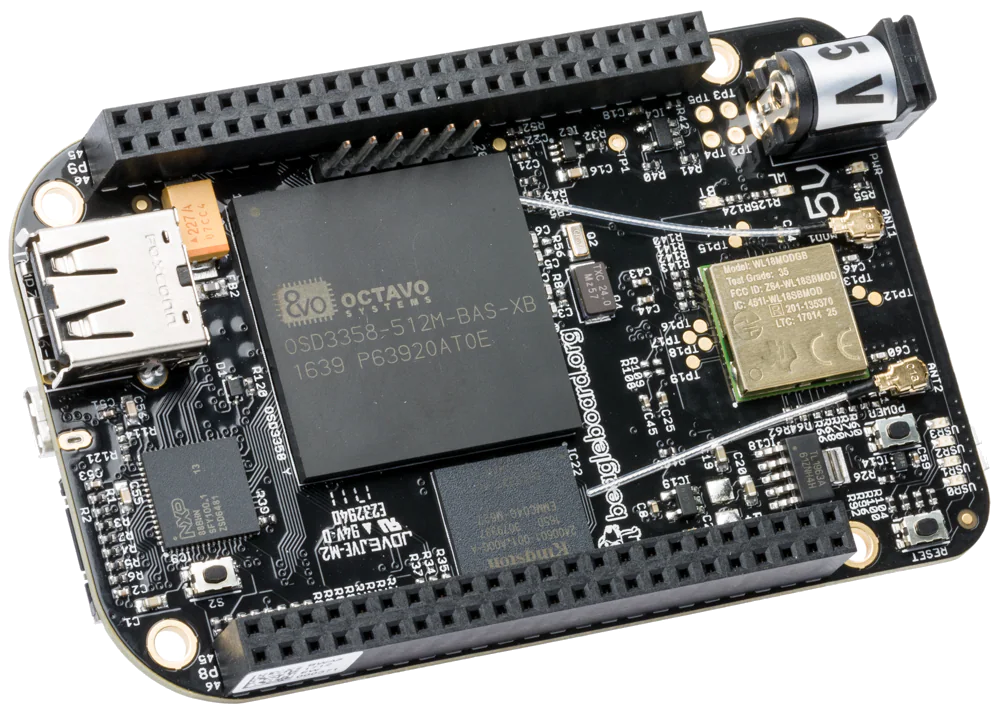
\includegraphics[width=5cm]{../slides/beagleboneblack-board/beagleboneblack.png}
  \end{center}
}

\feagendatwocolumn
{Plateforme matérielle pour les démonstrations, option \#2}
{
  Carte {\bf STMicroelectronics STM32MP157D Discovery Kit 1}
  \begin{itemize}
  \item Processeur STM32MP157D (double Cortex-A7) de STMicroelectronics
  \item Alimentée par USB
  \item 512 Mo DDR3L RAM
  \item Port Gigabit Ethernet port
  \item 4 ports hôte USB 2.0
  \item 1 port USB-C OTG
  \item 1 connecteur Micro SD
  \item Debugger ST-LINK/V2-1 sur la carte
  \item Connecteurs compatibles Arduino Uno v3
  \item Codec audio
  \item Divers: boutons, LEDs
  \end{itemize}
}
{}
{
  \begin{center}
    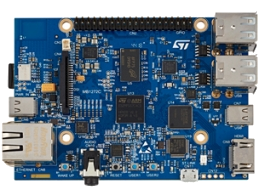
\includegraphics[width=5cm]{../slides/discovery-board-dk1/discovery-board-dk1.png}
  \end{center}
}

\section{1\textsuperscript{ère} demi-journée}

\feagendaonecolumn
{Cours – Introduction à Linux embarqué}
{
  \begin{itemize}
  \item Introduction au Logiciel Libre
  \item Atouts du Logiciel Libre pour les systèmes embarqués
  \item Exemples de systèmes embarqués fonctionnant sous Linux
  \item Besoins en CPU, RAM et stockage
  \item Choix d'une plateforme matérielle
  \item Architecture du système: composants principaux
  \item Différentes tâches pour développer un système embarqué
  \end{itemize}
}

\feagendatwocolumn
{Cours - Chaîne de compilation croisée et bibliothèque standard C}
{
  \begin{itemize}
  \item Les composants d'une chaîne de compilation croisée.
  \item Choisir une bibliothèque standard C.
  \item Le contenu de la bibliothèque standard C.
  \item Les chaînes de compilation croisée prêtes à l'emploi.
  \item La construction automatisée d'une chaîne de compilation croisée.
  \end{itemize}
}
{TP – Chaîne de compilation croisée}
{
  \begin{itemize}
  \item Configuration de Crosstool-NG
  \item Exécution pour construire une chaîne de compilation croisée
    personnalisée reposant sur la uClibc.
  \item Exploration du contenu d'une chaîne de compilation croisée
  \end{itemize}
}

\feagendaonecolumn
{Cours – Processus de démarrage, firmware, chargeurs de démarrage}
{
  \begin{itemize}
  \item Processus de démarrage des systèmes embarqués, focus sur les
    architectures {\em x86} et {\em ARM}
  \item Processus de démarrage et chargeurs de démarrage sur
    plateformes {\em x86} (legacy et UEFI)
  \item Processus de démarrage sur plateformes {\em ARM}: code en ROM,
    chargeurs de démarrage, {\em ARM Trusted Firmware}
  \item Focus sur U-Boot: configuration, installation et utilisation
  \item Commandes U-Boot, environnement U-Boot, scripts U-Boot,
    mécanisme {\em distro boot command} de U-Boot
  \end{itemize}
}

\section{2\textsuperscript{ème} demi-journée}

\feagendaonecolumn
{TP - U-Boot}
{
  \begin{itemize}
  \item Mise en place de la communication série avec la carte.
  \item Configuration, compilation et installation d'U-Boot sur la
    plateforme embarquée.
  \item Familiarisation avec l'environnement et les commandes
    d'U-Boot.
  \item Mise en place de la communication TFTP avec la carte.
    Utilisation des commandes TFTP d'U-Boot.
  \end{itemize}

  \vspace{0.5cm}
  {\em Mise en oeuvre sur la plateforme embarquée.}
}

\feagendatwocolumn
{Cours – Noyau Linux}
{
  \begin{itemize}
  \item Rôle et architecture générale du noyau Linux.
  \item Séparation entre noyau et espace utilisateur, interfaces entre
    l'espace utilisateur et le noyau
  \item Comprendre les différentes versions du noyau Linux: choix
    entre versions proposées par les fabricants et la version {\em
      upstream}, versions {\em Long Term Support}
  \item Récupérer les sources du noyau Linux
  \item Configuration du noyau Linux: configuration pré-définies,
    interfaces de configuration
  \item Concept de {\em Device Tree}
  \item Cross-compilation du noyau Linux
  \item Rôle des fichiers résultants de la compilation du noyau Linux
  \item Installation et démarrage du noyau Linux
  \item La ligne de commande du noyau Linux
  \end{itemize}
}
{TP - Compilation croisée du noyau et démarrage sur la carte}
{
  \begin{itemize}
  \item Configuration du noyau Linux et compilation croisée pour la
    plateforme embarquée.
  \item Téléchargement du noyau en utilisant le client TFTP d'U-Boot.
  \item Démarrage du noyau depuis la RAM.
  \item Automatisation du démarrage du noyau avec des scripts U-Boot.
  \end{itemize}

  \vspace{0.5cm}
  {\em Mise en oeuvre sur la plateforme embarquée.}
}

\section{3\textsuperscript{ème} demi-journée}

\feagendatwocolumn
{Cours – Système de fichier racine}
{
  \begin{itemize}
  \item Les systèmes de fichiers dans Linux.
  \item Rôle et organisation du système de fichiers racine.
  \item Localisation de ce système de fichiers: sur espace
	de stockage, en mémoire, sur le réseau.
  \item Les fichiers device, les systèmes de fichiers virtuels.
  \item Contenu type d'un système de fichiers racine.
  \end{itemize}
}
{Cours - BusyBox}
{
  \begin{itemize}
  \item Présentation de BusyBox. Intérêt pour les systèmes embarqués.
  \item Configuration, compilation et installation.
  \end{itemize}
}

\feagendaonecolumn
{TP – Construction d'un minuscule système Linux embarqué avec BusyBox}
{
  \begin{itemize}
  \item Construction à partir de zéro d'un système de fichiers racine
    contenant un système Linux embarqué
  \item Mise en place d'un noyau permettant de démarrer le système
    depuis un répertoire mis à disposition par la station de
    développement au travers de NFS.
  \item Passage de paramètres au noyau pour le démarrage avec NFS.
  \item Création complète du système de fichiers à partir de zéro :
    installation de BusyBox, création des fichiers spéciaux pour les
    périphériques.
  \item Initialisation du système en utilisant le programme init de BusyBox.
  \item Utilisation du serveur HTTP de BusyBox.
  \item Contrôle de la cible à partir d'un navigateur Web sur la
    station de développement.
  \item Mise en place des bibliothèques partagées sur la cible et
    développement d'une application d'exemple.
  \end{itemize}

  \vspace{0.5cm}
  {\em Mise en oeuvre sur la plateforme embarquée.}
}

\section{4\textsuperscript{ème} demi-journée}

\feagendatwocolumn
{Cours - Accès aux périphériques matériels}
{
  \begin{itemize}
  \item Comment accéder au matériel sur les principaux bus: USB, SPI,
    I2C, PCI
  \item Utilisation de pilotes de périphériques dans le noyau ou accès
    depuis l'espace utilisateur
  \item La syntaxe du {\em Device Tree}, et comment l'utilisation pour
    décrire des périphériques additionnels et le multiplexage des
    signaux.
  \item Trouver des pilotes de périphériques dans le noyau Linux pour
    des périphériques matériels.
  \item Utilisation de modules noyau
  \item Accès au matériel par \code{/dev} ou \code{sysfs}
  \item Interfaces en espace utilisateur pour les périphériques les
    plus courants: stockage, réseau, GPIO, LEDs, audio, affichage,
    video
  \end{itemize}
}
{TP - Accès aux périphériques matériels}
{
  \begin{itemize}
  \item Exploration du contenu de \code{/dev} et \code{sysfs}, et des
    périphériques disponibles sur la plateforme embarquée.
  \item Utilisation de GPIOs et de LEDs
  \item Modification du Device Tree pour ajouter le support pour un
    joystick connecté sur I2C
  \item Ajout du support pour une carte son USB en utilisant des
    modules noyau
  \end{itemize}

  \vspace{0.5cm}
  {\em Mise en oeuvre sur la plateforme embarquée.}
}

\feagendatwocolumn
{Cours - Système de fichiers bloc}
{
  \begin{itemize}
  \item Accéder et partitionner des périphériques bloc.
  \item Systèmes de fichiers pour périphériques bloc.
  \item Utilité des systèmes de fichiers journalisés.
  \item Systèmes de fichiers en lecture seule.
  \item Systèmes de fichiers en RAM.
  \item Création de chacun de ces systèmes de fichiers.
  \item Suggestions pour les systèmes embarqués.
  \end{itemize}
}
{TP - Système de fichiers bloc}
{
  \begin{itemize}
  \item Créer des partitions sur le stockage bloc.
  \item Démarrage d'un système avec un assemblage de plusieurs systèmes
    de fichiers : SquashFS pour les applications, ext3 pour la
    configuration et les données utilisateur et tmpfs pour les
    fichiers temporaires.
  \end{itemize}
  \vspace{0.5cm}
  {\em Mise en oeuvre sur la plateforme embarquée.}
}

\section{5\textsuperscript{ème} demi-journée}

\feagendaonecolumn
{Cours - Système de fichiers pour flash}
{
  \begin{itemize}
  \item Le sous-système Memory Technology Devices du noyau Linux.
  \item Les systèmes de fichiers pour le stockage MTD : JFFS2, YAFFS2,
    UBIFS.
  \item Options de configuration du noyau.
  \item Partitions MTD.
  \item Étude en détail de UBI et UBIFS: préparation, flashage et mise
    en oeuvre d'images UBI.
  \end{itemize}

  \vspace{0.5cm}

  {\em Note: la plateforme embarquée utilisée pour les labs ne
    comportant pas de mémoire flash NAND en accès direct, cette partie
    du cours ne sera pas illustrée avec un TP correspondant.}
}

\feagendatwocolumn
{Cours – Cross-compilation de bibliothèques et d'applications espace utilisateur}
{
  \begin{itemize}
  \item Configuration, compilation croisée et installation
    d'applications et de bibliothèques
  \item Concept de {\em build system}, et aperçu de quelques {\em
      build systems} courants utilisés dans les projets open-source:
    {\em Makefile}, {\em autotools}, {\em CMake}, {\em meson}
  \item Aperçu des problématiques courantes rencontrées lors de la
    compilation croisée
  \end{itemize}
}
{TP – Compilation croisée de bibliothèques et d'applications}
{
  \begin{itemize}
  \item Compilation croisée manuelle de plusieurs bibliothèques et
    applications open-source pour une plateforme embarquée.
  \item Apprentissage des principales techniques et des problèmes
    principaux.
  \end{itemize}

  \vspace{0.5cm}
  {\em Mise en oeuvre sur la plateforme embarquée.}
}

\section{6\textsuperscript{ème} demi-journée}

\feagendatwocolumn
{Cours - Outils de construction de systèmes}
{
  \begin{itemize}
  \item Les différentes approches pour construire un système Linux
    embarqué: {\em build systems} et distributions binaires
  \item Principe d'un {\em build system}, aperçu de Yocto
    Project/OpenEmbedded et de Buildroot
  \item Principe d'une {\em distribution binaire} et outils associés,
    focus sur Debian et Ubuntu
  \item Piles logicielles standards: Tizen, AGL, Android
  \end{itemize}
}
{TP - Construction d'un système avec Buildroot}
{
  \begin{itemize}
  \item Utilisation de Buildroot pour construire de façon automatisée
    un système similaire à celui du TP précédent.
  \item Voir à quel point cela est plus simple
  \item Optionnel: rajout d'un paquet dans Buildroot
  \end{itemize}

  \vspace{0.5cm}
  {\em Mise en oeuvre sur la plateforme embarquée.}
}

\feagendaonecolumn
{Cours - Licences open-source et mise en conformité}
{
  \begin{itemize}
  \item Présentation des principales licenses open-source: GPL, LGPL,
    MIT, BSD, Apache, etc.
  \item Concept de {\em copyleft} dans les licences open-source
  \item Différence entre (L)GPL version 2 et 3
  \item Mise en conformité avec les licences open-source: bonnes
    pratiques
  \end{itemize}
}

\feagendaonecolumn
{Cours - Aperçu des stack logicielles open-source majeurs pour Linux embarqué}
{
  \begin{itemize}
  \item \code{systemd} comme système {\em init}
  \item Gestion du matériel avec {\em udev}
  \item Communication inter-processus avec {\em D-Bus}
  \item La stack logicielle pour la connectivité: Ethernet, WiFi,
    modems, Bluetooth
  \item La stack logicielle pour le graphique: DRM/KMS, X.org,
    Wayland, Qt, Gtk, OpenGL
  \item La stack logicielle pour le multimédia: Video4Linux,
    GStreamer, Pulseaudio, Pipewire
  \end{itemize}
}

\section{7\textsuperscript{ème} jour - Matin}

\feagendaonecolumn
{TP - Intégration de stack logicielles additionnelles}
{
  \begin{itemize}
  \item Intégration de {\em systemd} comme système d'init
  \item Utilisation de {\em udev} pour le chargement automatique de
    modules
  \item Utilisation de {\em D-Bus} pour la communication
    inter-processus
  \item Intégration d'un player audio.
  \end{itemize}

  \vspace{0.5cm}
  {\em Mise en oeuvre sur la plateforme embarquée.}
}

\feagendaonecolumn
{Cours - Développement et déboguage d'application}
{
  \begin{itemize}
  \item Langages de programmations et bibliothèques disponibles.
  \item {\em Build system} pour votre application, un aperçu de {\em
      CMake} et {\em Meson}
  \item Le débogueur {\em gdb}: déboguage d'applications à distance
    avec gdb et gdbserver, analyse post-mortem d'une application.
  \item Analyse de performance, outils de {\em tracing} et {\em
      profiling}, analyseurs mémoire: \code{strace}, \code{ltrace},
    \code{perf}, \code{valgrind}
  \end{itemize}
}

\feagendaonecolumn
{TP – Développement et déboguage d'application}
{
  \begin{itemize}
  \item Création d'une application qui utilise un joystick connecté
    sur I2C pour contrôler un player audio.
  \item Mise en place d'un IDE pour le développement et le déboguage
    d'une application.
  \item Utilisation de {\em strace}, {\em ltrace}, {\em gdbserver} et
    {\em perf} pour déboguer/investiguer des applications
    problématiques sur la plateforme embarquée.
  \end{itemize}
  {\em Mise en oeuvre sur la plateforme embarquée.}
}

\end{document}
